\documentclass[11pt,a4paper]{article}

% ------------------------------------------------------------------
% Packages
% ------------------------------------------------------------------
\usepackage[margin=2.3cm]{geometry}
\usepackage[T1]{fontenc}
\usepackage{lmodern}
\usepackage{microtype}
\usepackage{xcolor}
\usepackage{graphicx}
\usepackage{booktabs}
\usepackage{tabularx}
\usepackage{array}
\usepackage{longtable}
\usepackage{enumitem}
\usepackage{listings}
\usepackage{tikz}
\usetikzlibrary{arrows.meta,positioning,shapes.geometric,fit,calc}
\usepackage[most]{tcolorbox}
\usepackage{fancyhdr}
\usepackage{titlesec}
\usepackage{caption}
\usepackage{needspace}
\usepackage{etoolbox}
\usepackage[hidelinks]{hyperref}
% Never leave a section heading alone at the bottom of a page.
\pretocmd{\section}{\needspace{14\baselineskip}}{}{}
\pretocmd{\subsection}{\needspace{8\baselineskip}}{}{}

% ------------------------------------------------------------------
% Colours and styles
% ------------------------------------------------------------------
\definecolor{mongo}{HTML}{13AA52}
\definecolor{mongodark}{HTML}{116149}
\definecolor{ink}{HTML}{102A43}
\definecolor{soft}{HTML}{F3F7FB}
\definecolor{line}{HTML}{D6E2ED}
\definecolor{kw}{HTML}{0866DC}
\definecolor{str}{HTML}{A3412F}
\definecolor{cmt}{HTML}{6B7F93}

\hypersetup{colorlinks=true,linkcolor=mongodark,urlcolor=kw}

\titleformat{\section}{\Large\bfseries\color{ink}}{\thesection}{0.8em}{}[{\color{mongo}\titlerule[1pt]}]
\titleformat{\subsection}{\large\bfseries\color{ink}}{\thesubsection}{0.7em}{}
\titleformat{\subsubsection}{\normalsize\bfseries\color{ink}}{\thesubsubsection}{0.6em}{}

\pagestyle{fancy}
\fancyhf{}
\fancyhead[L]{\small\color{cmt}ScoreStream}
\fancyhead[R]{\small\color{cmt}\nouppercase{\leftmark}}
\fancyfoot[C]{\small\thepage}
\renewcommand{\headrulewidth}{0.4pt}

\setlength{\parskip}{0.55em}
\setlength{\parindent}{0pt}
\renewcommand{\arraystretch}{1.25}

\lstdefinelanguage{JavaScript}{
  keywords={const,let,var,function,return,if,else,for,of,in,await,async,new,throw,try,catch,true,false,null,require},
  sensitive=true,
  comment=[l]{//},
  morecomment=[s]{/*}{*/},
  morestring=[b]',
  morestring=[b]",
  morestring=[b]`,
}
\lstset{
  language=JavaScript,
  basicstyle=\ttfamily\footnotesize\color{ink},
  keywordstyle=\color{kw}\bfseries,
  stringstyle=\color{str},
  commentstyle=\color{cmt}\itshape,
  backgroundcolor=\color{soft},
  frame=single,
  rulecolor=\color{line},
  framesep=6pt,
  xleftmargin=6pt,
  xrightmargin=6pt,
  breaklines=true,
  columns=fullflexible,
  keepspaces=true,
  showstringspaces=false,
  tabsize=2,
  aboveskip=0.8em,
  belowskip=0.8em,
}

\newcommand{\op}[1]{\texttt{\$#1}}
\newcommand{\coll}[1]{\texttt{#1}}

\newtcolorbox{viva}[1][]{colback=mongo!6,colframe=mongo,boxrule=0.6pt,arc=2pt,left=6pt,right=6pt,top=4pt,bottom=4pt,fonttitle=\bfseries\small,title={Viva point#1}}
\newtcolorbox{keyidea}{colback=kw!5,colframe=kw!70,boxrule=0.6pt,arc=2pt,left=6pt,right=6pt,top=4pt,bottom=4pt}

\tikzset{
  box/.style={draw=ink!60,rounded corners=3pt,fill=soft,align=center,font=\small,inner sep=6pt},
  mbox/.style={draw=mongodark,rounded corners=3pt,fill=mongo!12,align=center,font=\small,inner sep=6pt},
  arr/.style={-{Stealth[length=2.4mm]},thick,color=ink!70},
  lbl/.style={font=\scriptsize,color=ink!80,align=center},
}

% ------------------------------------------------------------------
\begin{document}

% ============================ TITLE PAGE ============================
\begin{titlepage}
  \centering
  \vspace*{1.5cm}
  {\color{mongo}\rule{\linewidth}{2pt}}\\[1.2em]
  {\Huge\bfseries\color{ink} ScoreStream}\\[0.6em]
  {\Large\color{ink} A Real-Time Event Judging System Built on MongoDB}\\[1.2em]
  {\color{mongo}\rule{\linewidth}{2pt}}\\[2.2em]
  {\large Project Report --- NoSQL Databases}\\[3em]

  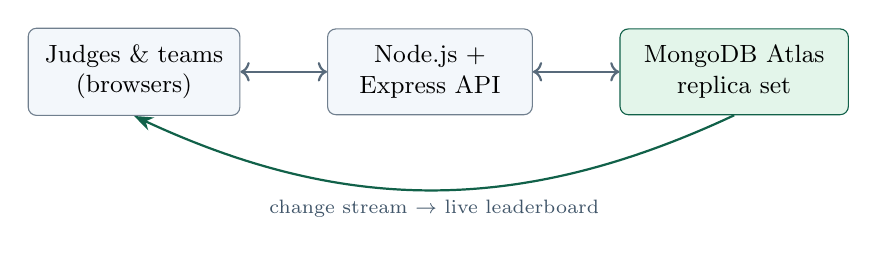
\begin{tikzpicture}[node distance=1.1cm]
    \node[box,minimum width=2.6cm] (b) {Judges \& teams\\(browsers)};
    \node[box,minimum width=2.6cm,right=of b] (n) {Node.js +\\Express API};
    \node[mbox,minimum width=2.9cm,right=of n] (m) {MongoDB Atlas\\replica set};
    \draw[arr,<->] (b) -- (n);
    \draw[arr,<->] (n) -- (m);
    \draw[arr,color=mongodark] (m.south) to[bend left=25] node[lbl,below]{change stream $\rightarrow$ live leaderboard} (b.south);
  \end{tikzpicture}

  \vfill
  \begin{tabular}{rl}
    \textbf{Prepared by:} & \rule{7cm}{0.4pt}\\[0.6em]
    \textbf{Roll number(s):} & \rule{7cm}{0.4pt}\\[0.6em]
    \textbf{Guide:} & \rule{7cm}{0.4pt}\\[0.6em]
    \textbf{Live site:} & \url{https://scorestream-rfqx.onrender.com}\\
  \end{tabular}\\[2em]
  {\small\color{cmt} Stack: MongoDB Atlas 8.0 (3-node replica set) $\cdot$ Node.js MongoDB driver v7 $\cdot$ Express 5 $\cdot$ HTML/JS}
\end{titlepage}

% ============================ ABSTRACT ============================
\section*{Abstract}
ScoreStream runs judged competitions such as hackathons and project expos. Organisers create events with a weighted
rubric, invite judges and teams by their permanent codes, judges score teams one at a time, and every team sees its
rank change live. When the event ends, an AI model turns the judges' short notes into written feedback.

This report concentrates on \textbf{how MongoDB is used}: where data lives in the cluster and how the
cluster keeps copies in sync, how documents are modelled, how unique judge and team codes are generated and why they
can never clash, which indexes exist and what they prove, every aggregation pipeline (\op{match}, \op{group},
\op{lookup}, \op{setWindowFields}, \op{merge}, \dots), how Change Streams push live updates, and how slide files
are stored with GridFS. Every number in the measurement tables was produced by running the real queries against the
real Atlas cluster.

\tableofcontents
\newpage

% ============================ 1 ============================
\section{Why MongoDB for this project}

\begin{itemize}[leftmargin=1.4em]
  \item \textbf{Each event has its own rubric.} One hackathon scores \emph{Innovation, Design, Execution}; another
        might score \emph{Idea, Pitch}. A score document simply stores \texttt{criteria: \{ innovation: 8, design: 7 \}}
        with whatever keys that event uses. In SQL this would need an extra criteria table and joins, or a schema change
        per event.
  \item \textbf{Data is read the way it is stored.} An event and its rubric are always needed together, so the rubric
        is \emph{embedded} inside the event document: one read, no join.
  \item \textbf{The database does the maths.} Averages, judge counts and competition ranks are produced by one
        \emph{aggregation pipeline} running inside MongoDB, and saved with \op{merge}.
  \item \textbf{Real-time out of the box.} \emph{Change Streams} tell the server the moment a score changes. There is
        no polling loop.
  \item \textbf{Files in the same database.} \emph{GridFS} stores the teams' slides, so no separate file server is
        needed and files survive server redeploys.
\end{itemize}

% ============================ 2 ============================
\section{MongoDB architecture: cluster, database, documents}

\subsection{The Atlas cluster is a replica set}
The data lives in a \textbf{MongoDB Atlas} cluster. We checked its shape with the \texttt{hello} command:
it is a \textbf{replica set of 3 members} running \textbf{MongoDB 8.0.34}.

\begin{center}
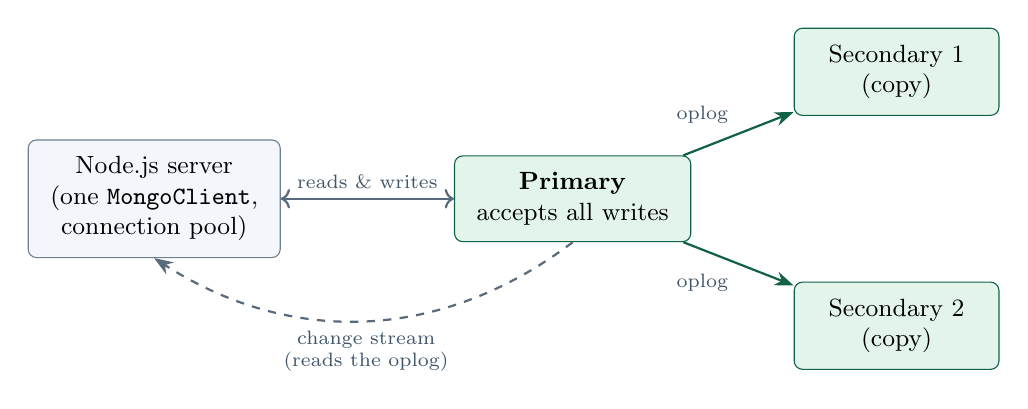
\begin{tikzpicture}[node distance=0.9cm and 1.6cm]
  \node[box,minimum width=3.2cm] (app) {Node.js server\\(one \texttt{MongoClient},\\connection pool)};
  \node[mbox,right=2.2cm of app,minimum width=3cm] (p) {\textbf{Primary}\\accepts all writes};
  \node[mbox,above right=0.5cm and 1.3cm of p,minimum width=2.6cm] (s1) {Secondary 1\\(copy)};
  \node[mbox,below right=0.5cm and 1.3cm of p,minimum width=2.6cm] (s2) {Secondary 2\\(copy)};
  \draw[arr,<->] (app) -- node[lbl,above]{reads \& writes} (p);
  \draw[arr,color=mongodark] (p) -- node[lbl,above left]{oplog} (s1);
  \draw[arr,color=mongodark] (p) -- node[lbl,below left]{oplog} (s2);
  \draw[arr,dashed] (p.south) to[bend left=35] node[lbl,below]{change stream\\(reads the oplog)} (app.south);
\end{tikzpicture}
\end{center}

\begin{itemize}[leftmargin=1.4em]
  \item \textbf{Primary}: every insert, update and delete goes here first.
  \item \textbf{Oplog} (operations log): the primary records each write in a special capped collection. The two
        \textbf{secondaries} copy the oplog and replay it, so all three hold the same data.
  \item \textbf{Automatic failover}: if the primary goes down, the secondaries elect a new primary within seconds and the
        driver reconnects by itself. The app keeps working.
  \item \textbf{Why we need a replica set}: Change Streams (Section~\ref{sec:sync}) are built on the oplog, so they only
        work on a replica set. Atlas clusters are always replica sets.
\end{itemize}

\subsection{How the server connects}
One \texttt{MongoClient} is created at start-up and reused by every request (\texttt{src/db.js}). The client keeps a
\textbf{connection pool} inside it, so requests do not pay the cost of opening a new connection.

\begin{lstlisting}
client = new MongoClient(config.mongodbUri);   // mongodb+srv://... from .env
await client.connect();
db = client.db(config.dbName);                 // database "judging_system"
await db.command({ ping: 1 });                 // proves the cluster answers
\end{lstlisting}

The connection string uses the \texttt{mongodb+srv://} scheme: the driver looks up DNS records to find all three
replica-set members automatically. The string (with the password) lives only in the server's \texttt{.env} file,
which is never committed to Git.

\subsection{Database $\rightarrow$ collections $\rightarrow$ documents}
\begin{itemize}[leftmargin=1.4em]
  \item \textbf{Database}: \texttt{judging\_system}. Tests use a separate \texttt{judging\_system\_test} database that is
        dropped after every run, so tests never touch real data.
  \item \textbf{Collection}: a group of documents, like a table, but without a fixed set of columns.
  \item \textbf{Document}: a JSON-like record stored as \textbf{BSON} (Binary JSON). BSON adds real types JSON lacks:
        \texttt{ObjectId}, \texttt{Date}, 64-bit integers and binary data. A score document averages \textbf{193 bytes}
        (measured with \texttt{collStats}).
  \item \textbf{\_id / ObjectId}: every document has a unique \texttt{\_id}. By default it is an \texttt{ObjectId}:
        12 bytes = a 4-byte \textbf{timestamp} + a 5-byte random value + a 3-byte counter. It is created by the
        driver, is unique without asking the server, and roughly sorts by creation time.
  \item \textbf{Storage engine}: \textbf{WiredTiger}, which stores documents compressed on disk and keeps the most used
        data and indexes in memory.
\end{itemize}

% ============================ 3 ============================
\section{Data model}

\subsection{The collections}
\begin{longtable}{@{}>{\ttfamily}p{3.3cm}p{6.2cm}p{5.6cm}@{}}
\toprule
\normalfont\textbf{Collection} & \textbf{Holds} & \textbf{Key fields}\\
\midrule
\endhead
events & One competition, with its rubric \emph{embedded} & name, status (draft/live/closed), rubric[], ownerId \\
admins & Organiser accounts & username, usernameLower, passwordHash \\
judgeAccounts & A registered judge (permanent) & name, \textbf{code} (JG\dots), passwordHash \\
teamAccounts & A registered team (permanent) & name, members[], \textbf{code} (TM\dots), passwordHash \\
judgeInvitations & Admin asks a judge to join an event & eventId, accountId, status, invitedBy \\
invitations & Admin asks a team to join an event & eventId, accountId, status, invitedBy \\
judges & A judge's \emph{seat} in one event & eventId, accountId, name, joinedAt \\
teams & A team's \emph{place} in one event & eventId, accountId, name, members[] \\
scores & One judge's marks for one team & eventId, teamId, judgeId, criteria\{\}, total, comment \\
leaderboard & Ranked results (written only by \op{merge}) & eventId, teamId, avgScore, judgesCount, rank \\
feedback & AI feedback per team & summary, strengths[], improvements[], sentiment \\
submissions & A team's GitHub link + slides info & eventId, teamId, githubUrl, slides\{fileId,\dots\} \\
slides.files / slides.chunks & \textbf{GridFS} file storage & the uploaded PDF/PPT bytes in 255\,KB chunks \\
\bottomrule
\end{longtable}

\subsection{How the collections reference each other}
\begin{center}
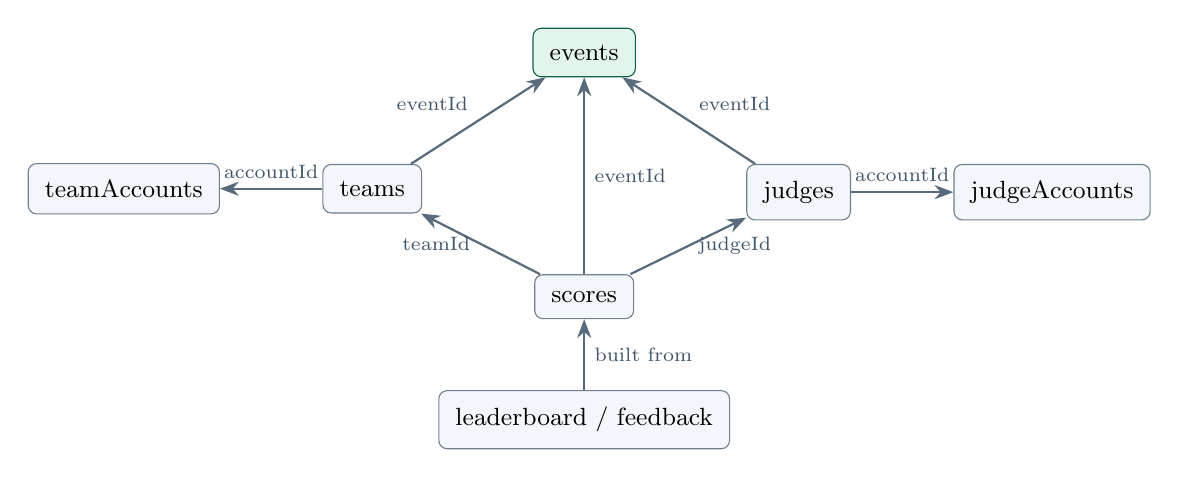
\begin{tikzpicture}[node distance=1.2cm and 1.5cm, every node/.style={font=\small}]
  \node[mbox] (ev) {events};
  \node[box,below left=1.1cm and 1.4cm of ev] (tm) {teams};
  \node[box,below right=1.1cm and 1.4cm of ev] (jd) {judges};
  \node[box,below=2.5cm of ev] (sc) {scores};
  \node[box,left=1.3cm of tm] (ta) {teamAccounts};
  \node[box,right=1.3cm of jd] (ja) {judgeAccounts};
  \node[box,below=0.9cm of sc] (lb) {leaderboard / feedback};
  \draw[arr] (tm) -- node[lbl,above left]{eventId} (ev);
  \draw[arr] (jd) -- node[lbl,above right]{eventId} (ev);
  \draw[arr] (tm) -- node[lbl,above]{accountId} (ta);
  \draw[arr] (jd) -- node[lbl,above]{accountId} (ja);
  \draw[arr] (sc) -- node[lbl,left]{teamId} (tm);
  \draw[arr] (sc) -- node[lbl,right]{judgeId} (jd);
  \draw[arr] (sc) -- node[lbl,right]{eventId} (ev);
  \draw[arr] (lb) -- node[lbl,right]{built from} (sc);
\end{tikzpicture}
\end{center}

\subsection{Embedding vs referencing --- the main design decision}
\begin{tabularx}{\linewidth}{@{}p{3.2cm}X@{}}
\toprule
\textbf{Choice} & \textbf{Why}\\
\midrule
Rubric \textbf{embedded} in the event & Small (3--6 items), always read with the event, never queried on its own. One read gives everything. \\
Scores \textbf{referenced} (own collection) & Written very often by many judges at once, queried on their own (per event, per team), and the count grows with teams $\times$ judges. Embedding them inside a team would create one hot, ever-growing document that every judge writes to. \\
Accounts vs.\ seats & A team or judge \emph{account} is permanent and can join many events; the \coll{teams}/\coll{judges} document is its seat in one event. Scores point at the seat, so removing a judge from one event never touches their other events. \\
\bottomrule
\end{tabularx}

\subsection{Example documents}
An \textbf{event} with its embedded rubric:
\begin{lstlisting}
{ "_id": ObjectId("6ade3fca77d4420e1b815c02"),
  "name": "Spring Hackathon", "status": "live",
  "rubric": [ { "key": "innovation", "label": "Innovation", "max": 10, "weight": 0.3 },
              { "key": "design",     "label": "Design",     "max": 10, "weight": 0.4 },
              { "key": "execution",  "label": "Execution",  "max": 10, "weight": 0.3 } ],
  "ownerId": ObjectId("..."), "createdAt": ISODate("2026-10-25T17:40:00Z") }
\end{lstlisting}

A \textbf{score} --- \texttt{criteria} keys follow the event's rubric:
\begin{lstlisting}
{ "eventId": ObjectId("..."), "teamId": ObjectId("..."), "judgeId": ObjectId("..."),
  "criteria": { "innovation": 10, "design": 6.5, "execution": 5 },
  "total": 7.1,
  "comment": "Ui is nice but laggy, the slides could have been better",
  "submittedAt": ISODate("2026-10-25T17:52:11Z") }
\end{lstlisting}

\textbf{Scoring formula} (computed on the server, never trusted from the browser):
\[
  \textit{total} \;=\; 10 \times \sum_i \frac{\textit{mark}_i}{\textit{max}_i}\times \textit{weight}_i
  \qquad\text{e.g. } 10\times(0.3\cdot\tfrac{10}{10} + 0.4\cdot\tfrac{6.5}{10} + 0.3\cdot\tfrac{5}{10}) = 7.1
\]

A \textbf{judge account}:
\begin{lstlisting}
{ "_id": ObjectId("..."), "name": "Prof. Rao", "code": "JG3H8M2P",
  "passwordHash": "9f2c...e1:5ab0...77",          // scrypt "salt:hash", never the password
  "createdAt": ISODate("2026-10-25T17:30:00Z") }
\end{lstlisting}

% ============================ 4 ============================
\section{Schema validation with \texorpdfstring{\$jsonSchema}{$jsonSchema}}
MongoDB is schemaless by default. We still want the \emph{database itself} to reject malformed data, even if a bug
in the Node code lets something through. \texttt{scripts/setup-db.js} attaches a \textbf{\op{jsonSchema} validator}
to all 12 collections with \texttt{validationLevel: "strict"} (check every insert and update) and
\texttt{validationAction: "error"} (reject, don't just warn).

\begin{lstlisting}
scores: { $jsonSchema: {
  bsonType: 'object',
  required: ['eventId', 'teamId', 'judgeId', 'criteria', 'total', 'submittedAt'],
  properties: {
    eventId:  { bsonType: 'objectId' },
    criteria: { bsonType: 'object', additionalProperties: { bsonType: 'number' } },
    total:    { bsonType: 'number', minimum: 0, maximum: 10 },
    comment:  { bsonType: 'string' } } } }

judgeAccounts: { $jsonSchema: { ... properties: {
    code:         { bsonType: 'string', pattern: '^JG[A-Z0-9]{6}$' },
    passwordHash: { bsonType: 'string', pattern: '^[a-f0-9]{32}:[a-f0-9]{128}$' } } } }
\end{lstlisting}

\begin{itemize}[leftmargin=1.4em]
  \item \texttt{criteria} accepts \emph{any} keys (each event's rubric differs) but \emph{only numbers} as values.
  \item The \texttt{passwordHash} pattern means a plain-text password can never be stored by mistake.
  \item \textbf{Proof}: inserting \texttt{criteria: \{ innovation: "ten" \}, total: 99} is refused by the server with
        \texttt{code 121: Document failed validation}.
  \item Rules a schema cannot express (\emph{weights add up to 1}, \emph{criteria keys match this event's rubric})
        are checked in Node before writing.
\end{itemize}

% ============================ 5 ============================
\section{Judge and team codes: generation and uniqueness}

\subsection{How a code is generated}
Every judge and team gets a permanent code: \texttt{JG} or \texttt{TM} followed by 6 characters, e.g.\
\texttt{JG3H8M2P}. The code is what the organiser types to invite them, and what they use to sign in (with their
password). From \texttt{src/middleware/auth.js}:

\begin{lstlisting}
// No 0/O or 1/I, so codes are easy to read out loud.
const CODE_LETTERS = 'ABCDEFGHJKLMNPQRSTUVWXYZ23456789';   // 32 characters

function generateAccountCode(prefix) {
  const bytes = crypto.randomBytes(6);        // cryptographically secure random bytes
  let code = prefix;
  for (const byte of bytes) code += CODE_LETTERS[byte % CODE_LETTERS.length];
  return code;
}
const generateJudgeCode = () => generateAccountCode('JG');
\end{lstlisting}

\begin{itemize}[leftmargin=1.4em]
  \item \texttt{crypto.randomBytes} comes from the operating system's secure generator (not \texttt{Math.random}),
        so codes cannot be predicted.
  \item 32 symbols, 6 positions: $32^6 = 1{,}073{,}741{,}824$ possible codes per prefix.
  \item A byte has 256 values and $256 = 8 \times 32$, so \texttt{byte \% 32} picks every symbol with exactly equal
        probability (no \emph{modulo bias}).
\end{itemize}

\subsection{How we make sure no two judges get the same code}
Random codes \emph{can} collide in theory. The guarantee comes from MongoDB, not from luck:

\begin{lstlisting}
// scripts/setup-db.js -- a UNIQUE index on the code
db.judgeAccounts.createIndex({ code: 1 }, { unique: true, name: 'unique_code' })
db.teamAccounts.createIndex({ code: 1 },  { unique: true, name: 'unique_code' })
\end{lstlisting}

With a unique index, the \emph{database} refuses a second document with an existing code and returns
\textbf{error 11000 (duplicate key)}. Registration simply tries again with a fresh code (\texttt{src/routes/auth.js}):

\begin{lstlisting}
async function insertWithCode(collection, account, makeCode) {
  for (let attempt = 1; ; attempt++) {
    account.code = makeCode();
    try {
      const result = await collection.insertOne(account);
      return result.insertedId;                       // code was free -> done
    } catch (err) {
      if (err.code !== 11000 || attempt >= 5) throw err; // 11000 = code already taken
      delete account._id;                             // retry with a new random code
    }
  }
}
\end{lstlisting}

\begin{keyidea}
\textbf{Why not ``check if the code exists, then insert''?} Two registrations at the same instant could both check,
both see the code is free, and both insert it --- a \emph{race condition}. A unique index is checked \emph{atomically
inside the insert}, so exactly one of them can win. The chance of even one retry is tiny: with 10{,}000 judges already
registered, a new random code clashes with probability $10{,}000 / 32^6 \approx 0.0009\%$.
\end{keyidea}

\textbf{Signing in} uses the same index to find the account instantly, then checks the password:
\begin{lstlisting}
const account = await db.collection('judgeAccounts').findOne({ code: code.trim().toUpperCase() });
if (!account || !checkPassword(password, account.passwordHash)) throw httpError(401, 'Wrong judge code or password');
\end{lstlisting}
Passwords are stored only as \textbf{scrypt} hashes with a random 16-byte salt, compared with
\texttt{crypto.timingSafeEqual}.

\subsection{No duplicate invitations, no judge added twice}
Joining an event is a two-step handshake, and both steps are protected by indexes:

\begin{enumerate}[leftmargin=1.6em]
  \item The admin enters the judge's code $\rightarrow$ a \coll{judgeInvitations} document with
        \texttt{status: "pending"}.
  \item The judge accepts on their dashboard $\rightarrow$ a \coll{judges} document (their seat) is inserted.
\end{enumerate}

\begin{lstlisting}
// At most ONE pending invitation per judge per event. PARTIAL index: only documents
// with status 'pending' are in it, so old accepted/declined invitations never clash.
db.judgeInvitations.createIndex({ eventId: 1, accountId: 1 },
  { unique: true, partialFilterExpression: { status: 'pending' } })

// A judge account can hold at most one seat per event.
db.judges.createIndex({ eventId: 1, accountId: 1 }, { unique: true })
\end{lstlisting}
Teams use exactly the same pattern (\coll{invitations} and \coll{teams}). Inviting the same judge twice, or clicking
\emph{Accept} twice in two tabs, ends in error 11000 instead of a duplicate.

\begin{viva}
``What stops a judge scoring the same team twice?'' --- The unique compound index
\texttt{\{eventId, teamId, judgeId\}} on \coll{scores}. We verified it: inserting a copy of an existing score returns
\texttt{E11000 duplicate key error \dots index: unique\_event\_team\_judge}. Editing a score uses
\texttt{findOneAndUpdate} on the existing document instead.
\end{viva}

% ============================ 6 ============================
\section{Indexes}

\subsection{All indexes}
\begin{longtable}{@{}>{\ttfamily}p{3.1cm}>{\ttfamily}p{5.4cm}p{6.6cm}@{}}
\toprule
\normalfont\textbf{Collection} & \normalfont\textbf{Index} & \textbf{Purpose}\\
\midrule
\endhead
scores & \{eventId, teamId, judgeId\} \textbf{unique} & One score per judge per team (no double scoring) \\
scores & \{eventId\} & Fast ``all scores of this event'' --- first stage of the leaderboard pipeline \\
leaderboard & \{eventId, teamId\} \textbf{unique} & Required by \op{merge} \texttt{on: [eventId, teamId]} \\
feedback & \{eventId, teamId\} \textbf{unique} & One AI review per team; regenerate = upsert \\
judgeAccounts & \{code\} \textbf{unique} & Unique judge codes + fast login \\
teamAccounts & \{code\} \textbf{unique} & Unique team codes + fast login \\
judges & \{eventId, accountId\} \textbf{unique} & A judge sits in an event once \\
judges & \{accountId\} & ``Which events does this judge judge?'' \\
teams & \{eventId, accountId\} \textbf{unique, partial} & A team joins an event once \\
judgeInvitations & \{eventId, accountId\} \textbf{unique, partial} & One \emph{pending} invite per judge per event \\
invitations & \{eventId, accountId\} \textbf{unique, partial} & One \emph{pending} invite per team per event \\
submissions & \{eventId, teamId\} \textbf{unique} & One submission per team per event \\
admins & \{usernameLower\} \textbf{unique} & ``Asha'' and ``asha'' can't both register \\
events & \{ownerId, createdAt: -1\} & An organiser's events, newest first \\
\bottomrule
\end{longtable}

\textbf{Index types used}: \emph{single-field}, \emph{compound} (several fields, order matters),
\emph{unique}, and \emph{partial} (only documents matching a filter are indexed).

\subsection{Proof: COLLSCAN vs IXSCAN}
\texttt{scripts/explain.js} runs \texttt{.explain("executionStats")} on our two most important queries. We ran it on a
copy of the schema with \textbf{500 scores} (5 events $\times$ 20 teams $\times$ 5 judges), once with the indexes and
once after dropping them:

\begin{center}
{\small\setlength{\tabcolsep}{5pt}
\begin{tabular}{@{}lllrrr@{}}
\toprule
\textbf{Query} & \textbf{Index} & \textbf{Plan (stages)} & \textbf{Returned} & \textbf{Keys read} & \textbf{Docs read}\\
\midrule
\texttt{find(\{eventId\})} & none & \texttt{COLLSCAN} & 100 & 0 & \textbf{500}\\
\texttt{find(\{eventId\})} & yes & \texttt{IXSCAN} $\rightarrow$ \texttt{FETCH} & 100 & 100 & \textbf{100}\\
Leaderboard pipeline & none & \texttt{COLLSCAN} $\rightarrow$ \texttt{GROUP} & 20 & 0 & \textbf{500}\\
Leaderboard pipeline & yes & \texttt{IXSCAN} $\rightarrow$ \texttt{FETCH} $\rightarrow$ \texttt{GROUP} & 20 & 100 & \textbf{100}\\
\bottomrule
\end{tabular}}
\end{center}
In both ``yes'' rows MongoDB chose the \texttt{eventId\_1} index.

Without the index MongoDB reads \emph{every} score in the collection (all events) to find one event's 100. With it,
it jumps straight to those 100. The difference grows with the data: with 100 events it would be 100 documents read
instead of 10{,}000. To reproduce: \mbox{\texttt{npm run explain -{}- -{}-drop-indexes}}, then
\texttt{npm run setup-db}, then \texttt{npm run explain}.

% ============================ 7 ============================
\section{CRUD operations used}
\begin{longtable}{@{}>{\ttfamily}p{3.6cm}p{11.4cm}@{}}
\toprule
\normalfont\textbf{Operation} & \textbf{Where it is used}\\
\midrule
\endhead
insertOne & Register an account, create an event, invitation, seat, submit a score \\
insertMany & Seeding test data \\
findOne & Log in by code; load an event; ``is this judge in this event?'' (\texttt{findJudgeSeat}) \\
find + projection + sort & Leaderboard rows sorted by rank; never sending \texttt{passwordHash} (\texttt{projection: \{passwordHash: 0\}}) \\
countDocuments & Number of teams in an event \\
updateOne + \$set & Answer an invitation (\texttt{status: "accepted"}, \texttt{respondedAt}) \\
findOneAndUpdate & Edit a score (filter includes \texttt{judgeId}, so a judge can only edit their own); change event status; \texttt{returnDocument: "after"} \\
upsert & Save a GitHub link / feedback: update if it exists, insert if not (\texttt{replaceOne(..., \{upsert: true\})}) \\
\$unset & Remove a GitHub link or slides from a submission \\
deleteMany & Cascade delete: removing an event deletes its teams, judges, scores, leaderboard, feedback, invitations (MongoDB has no \texttt{ON DELETE CASCADE}) \\
\bottomrule
\end{longtable}

% ============================ 8 ============================
\section{Aggregation pipelines}
An aggregation pipeline is a list of \textbf{stages}. Documents flow through them in order and each stage transforms
the stream: filter, group, join, sort, rank, reshape, write. The work runs \emph{inside the database}, next to the
data, instead of loading everything into Node.

\subsection{The leaderboard pipeline (\texttt{src/services/leaderboard.js})}
This is the heart of the project: it turns raw scores into a ranked leaderboard.

\begin{center}
\resizebox{\linewidth}{!}{%
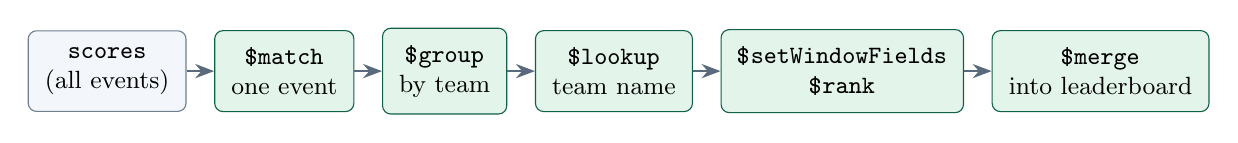
\begin{tikzpicture}[node distance=0.35cm]
  \node[box] (s0) {\coll{scores}\\(all events)};
  \node[mbox,right=of s0] (s1) {\op{match}\\one event};
  \node[mbox,right=of s1] (s2) {\op{group}\\by team};
  \node[mbox,right=of s2] (s3) {\op{lookup}\\team name};
  \node[mbox,right=of s3] (s4) {\op{setWindowFields}\\\op{rank}};
  \node[mbox,right=of s4] (s5) {\op{merge}\\into leaderboard};
  \foreach \a/\b in {s0/s1,s1/s2,s2/s3,s3/s4,s4/s5} \draw[arr] (\a) -- (\b);
\end{tikzpicture}}
\end{center}

\begin{lstlisting}
[
  // 1. $match FIRST: only this event's scores. Uses the { eventId: 1 } index (IXSCAN),
  //    so every later stage works on fewer documents.
  { $match: { eventId } },

  // 2. $group: one output document per team.
  { $group: { _id: '$teamId',
              avgScore:    { $avg: '$total' },   // average of every judge's total
              judgesCount: { $sum: 1 } } },       // +1 per score = number of judges

  // Round BEFORE ranking, so two teams showing 7.25 share a rank.
  { $set: { avgScore: { $round: ['$avgScore', 2] } } },

  // 3. $lookup = join with teams to get the name (scores store only teamId).
  { $lookup: { from: 'teams', localField: '_id', foreignField: '_id', as: 'team' } },
  { $unwind: '$team' },        // [ {team} ] -> {team}; drops scores of deleted teams

  // 4. Window function: rank by average, highest first. Ties share a rank: 1, 2, 2, 4.
  { $setWindowFields: { sortBy: { avgScore: -1 }, output: { rank: { $rank: {} } } } },

  // Shape each row like a leaderboard document.
  { $project: { _id: 0, eventId: { $literal: eventId }, teamId: '$_id', teamName: '$team.name',
                avgScore: 1, judgesCount: 1, rank: 1, updatedAt: { $literal: now } } },

  // 5. $merge: write the rows into the leaderboard collection.
  { $merge: { into: 'leaderboard', on: ['eventId', 'teamId'],
              whenMatched: 'replace', whenNotMatched: 'insert' } }
]
\end{lstlisting}

\subsubsection*{What each stage does}
\begin{tabularx}{\linewidth}{@{}>{\ttfamily}p{3.1cm}X@{}}
\toprule
\normalfont\textbf{Stage} & \textbf{Meaning}\\
\midrule
\$match & Filter, like SQL \texttt{WHERE}. Placed first so it can use an index. \\
\$group & Like SQL \texttt{GROUP BY}. \texttt{\_id} is the grouping key; accumulators \op{avg}, \op{sum} compute per group. \\
\$set / \$round & Add or overwrite a field; round to 2 decimals. \\
\$lookup & Left outer join with another collection; the matches arrive as an array. \\
\$unwind & One output document per array element (turns \texttt{[team]} into \texttt{team}). \\
\$setWindowFields & Window function (MongoDB 5.0+): computes a value using neighbouring documents --- here \op{rank} over the sorted list. \\
\$project & Choose, rename and compute output fields (like SQL \texttt{SELECT}). \\
\$merge & Write results into a collection, updating matching rows (needs a unique index on the \texttt{on} fields). \\
\bottomrule
\end{tabularx}

\subsubsection*{Worked example}
Real output from the 500-score test data (event 3, 20 teams, 5 judges each):
\begin{center}
\begin{tabular}{@{}cllc@{}}
\toprule
\textbf{rank} & \textbf{teamName} & \textbf{avgScore} & \textbf{judgesCount}\\
\midrule
1 & Team 3-6 & 7.9 & 5\\
2 & Team 3-12 & 7.3 & 5\\
3 & Team 3-16 & 7.1 & 5\\
4 & Team 3-18 & 6.7 & 5\\
\bottomrule
\end{tabular}
\end{center}

\begin{viva}
\textbf{\op{merge} vs \op{out}}: \op{out} replaces the \emph{whole} target collection, which would wipe every other
event's leaderboard. \op{merge} updates only the matching rows (\texttt{on: [eventId, teamId]}). Rows that
\op{merge} did not touch (a team whose scores were all deleted) are removed afterwards with
\texttt{deleteMany(\{ eventId, updatedAt: \{ \$lt: now \} \})}.
\end{viva}

\subsection{Per-criterion averages for a team (\op{objectToArray})}
The team page shows ``Design 6.5/10, Innovation 10/10\dots''. Because \texttt{criteria} is an object with
event-specific keys, we first turn it into an array of key/value pairs:
\begin{lstlisting}
[ { $match:   { eventId, teamId } },
  // { design: 6.5, innovation: 10 }  ->  [ {k:'design', v:6.5}, {k:'innovation', v:10} ]
  { $project: { pairs: { $objectToArray: '$criteria' } } },
  // one document per key/value pair
  { $unwind:  '$pairs' },
  // average mark per criterion
  { $group:   { _id: '$pairs.k', avg: { $avg: '$pairs.v' } } } ]
\end{lstlisting}

\subsection{Counting without copying: \op{lookup} with a sub-pipeline}
The admin's event list shows how many teams, judges and scores each event has. A \op{lookup} with its own
\texttt{pipeline} that ends in \op{count} returns just a number, without copying hundreds of documents:
\begin{lstlisting}
{ $lookup: { from: 'scores',
             let: { id: '$_id' },
             pipeline: [ { $match: { $expr: { $eq: ['$eventId', '$$id'] } } },
                         { $count: 'n' } ],
             as: 'scores' } },
{ $set: { scoreCount: { $ifNull: [ { $first: '$scores.n' }, 0 ] } } }
\end{lstlisting}
\texttt{\$\$id} refers to the variable defined in \texttt{let}; \op{expr} lets a \op{match} compare two fields.

\subsection{Other pipelines in the app}
\begin{tabularx}{\linewidth}{@{}p{4.1cm}X@{}}
\toprule
\textbf{Pipeline} & \textbf{Stages}\\
\midrule
Judge dashboard & \op{match} seats by accountId $\rightarrow$ \op{lookup} events $\rightarrow$ \op{lookup}+\op{count} teams and own scores $\rightarrow$ \op{project} progress \\
Judges list (admin) & \op{match} event $\rightarrow$ \op{lookup} judgeAccounts (code) $\rightarrow$ \op{lookup}+\op{count} scores per judge \\
Team dashboard & \op{match} by accountId $\rightarrow$ \op{lookup} events $\rightarrow$ \op{lookup} leaderboard with \texttt{let} + \op{expr} on two fields $\rightarrow$ \op{project} rank \\
Judges' scores for a team & \op{match} $\rightarrow$ \op{lookup} judges (names) $\rightarrow$ \op{project} with \op{ifNull} $\rightarrow$ \op{sort} \\
Teams for a judge & \op{match} event $\rightarrow$ \op{lookup} submissions $\rightarrow$ \op{set} githubUrl/slides with \op{first} $\rightarrow$ \op{project} hiding internal ids \\
Pending invitations & \op{match} \texttt{status: "pending"} $\rightarrow$ \op{lookup} events/accounts $\rightarrow$ \op{unwind} $\rightarrow$ \op{sort} \\
\bottomrule
\end{tabularx}

% ============================ 9 ============================
\section{Real-time synchronisation: Change Streams}\label{sec:sync}

\subsection{From a judge's click to every screen}
\begin{center}
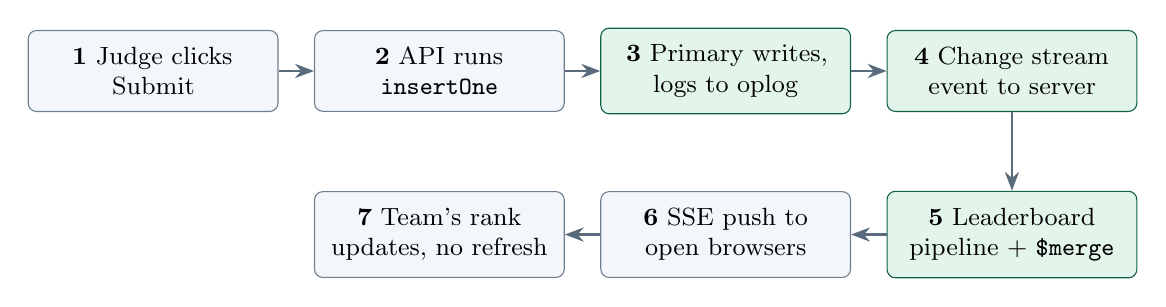
\begin{tikzpicture}[node distance=0.45cm]
  \node[box,text width=2.75cm] (a) {\textbf{1} Judge clicks\\Submit};
  \node[box,text width=2.75cm,right=of a] (b) {\textbf{2} API runs\\\texttt{insertOne}};
  \node[mbox,text width=2.75cm,right=of b] (c) {\textbf{3} Primary writes,\\logs to oplog};
  \node[mbox,text width=2.75cm,right=of c] (d) {\textbf{4} Change stream\\event to server};
  \node[mbox,text width=2.75cm,below=1cm of d] (e) {\textbf{5} Leaderboard\\pipeline + \op{merge}};
  \node[box,text width=2.75cm,left=of e] (f) {\textbf{6} SSE push to\\open browsers};
  \node[box,text width=2.75cm,left=of f] (g) {\textbf{7} Team's rank\\updates, no refresh};
  \draw[arr] (a)--(b); \draw[arr] (b)--(c); \draw[arr] (c)--(d); \draw[arr] (d)--(e); \draw[arr] (e)--(f); \draw[arr] (f)--(g);
\end{tikzpicture}
\end{center}

\subsection{The change stream (\texttt{src/services/changeStream.js})}
\begin{lstlisting}
stream = db.collection('scores').watch(
  // A pipeline that runs INSIDE MongoDB: only these 4 kinds of change are sent to us.
  [ { $match: { operationType: { $in: ['insert', 'update', 'replace', 'delete'] } } } ],
  // For updates, also send the whole updated document (we need its eventId).
  { fullDocument: 'updateLookup' }
);

stream.on('change', (change) => {
  // Handle changes one at a time, in order, so two recomputes never race.
  queue = queue.then(() => handleChange(change));
});
\end{lstlisting}

\begin{itemize}[leftmargin=1.4em]
  \item \texttt{watch()} opens a cursor on the \textbf{oplog}. MongoDB \emph{pushes} each change to the server ---
        the server never polls the database.
  \item \texttt{handleChange} reads \texttt{change.fullDocument.eventId} and recomputes \emph{only that event's}
        leaderboard. A \texttt{delete} event carries only the deleted \texttt{\_id}, so in that case every live event
        is recomputed.
  \item The handler writes to \coll{leaderboard}, never to \coll{scores}. Writing to the watched collection would
        trigger itself again in an endless loop.
  \item The result is pushed to browsers with \textbf{Server-Sent Events} (one long-lived HTTP response per open page;
        the browser's \texttt{EventSource} reconnects by itself). A heartbeat every 25\,s keeps proxies from closing
        idle connections.
\end{itemize}

\subsection{What else is synchronised live}
\begin{tabularx}{\linewidth}{@{}p{4.4cm}X@{}}
\toprule
\textbf{Event} & \textbf{Who updates without refreshing}\\
\midrule
A score is saved or edited & Team: rank, average, judges' marks. Admin: rankings, judging progress. Public leaderboard. \\
Admin sets Live / ends the event & Judge: stars unlock or lock. Team: status, submission lock. \\
A team or judge accepts an invitation & Admin: the team/judge appears in the event's list. Judge: a new team appears. \\
AI feedback is written & Team: the feedback card fills in. \\
\bottomrule
\end{tabularx}

\subsection{Consistency guarantees}
\begin{itemize}[leftmargin=1.4em]
  \item \textbf{Single-document atomicity}: every write in MongoDB is atomic per document, so a score is never
        half-saved.
  \item \textbf{Constraints in the database}: unique indexes and \op{jsonSchema} validators are enforced by the
        server for \emph{every} client, even if two requests arrive at the same millisecond.
  \item \textbf{Durability}: writes are acknowledged by a majority of the replica set (the Atlas default write concern
        \texttt{w: "majority"}), so an acknowledged score survives the loss of the primary.
  \item \textbf{Ordered processing}: change events are handled one after another through a promise queue.
\end{itemize}

% ============================ 10 ============================
\section{File storage with GridFS}
Teams upload slides (PDF, PowerPoint, Word, Excel, images, up to 20\,MB). A single MongoDB document is limited to
16\,MB, so files are stored with \textbf{GridFS}, MongoDB's built-in file system:

\begin{itemize}[leftmargin=1.4em]
  \item \coll{slides.chunks}: the file split into \textbf{255\,KB chunks} (a 2.9\,MB PDF became 12 chunks).
  \item \coll{slides.files}: one document per file: name, length, upload date and our metadata (eventId, teamId,
        content type).
  \item \coll{submissions}: the team's document points at the file through \texttt{slides.fileId}.
\end{itemize}

\begin{lstlisting}
const bucket = new GridFSBucket(db, { bucketName: 'slides' });
const upload = bucket.openUploadStream(filename, { metadata: { eventId, teamId, contentType } });
// The request body is STREAMED into GridFS chunk by chunk (never the whole file in memory),
// through a Transform that aborts once 20 MB is exceeded.
await pipeline(req, sizeLimit, upload);
\end{lstlisting}

Files live in the database, so they are replicated to all three members and survive server redeploys (the hosting
platform's own disk is wiped on every deploy). Replacing slides deletes the old file only \emph{after} the new one is
saved; deleting an event deletes its files too.

% ============================ 11 ============================
\section{Security and data protection}
\begin{itemize}[leftmargin=1.4em]
  \item Passwords: \textbf{scrypt} hash with a random salt; the validator pattern forbids plain text.
  \item Queries never return secrets: \texttt{projection: \{ passwordHash: 0 \}}.
  \item Every request is authorised against the database: a judge can score only teams of an event where they hold a
        seat (\texttt{findOne(\{ eventId, accountId \})}), and only while the event is \texttt{live}; an organiser can
        manage only events whose \texttt{ownerId} is theirs.
  \item The connection string and API keys live in \texttt{.env}, which is excluded from Git.
  \item Atlas encrypts connections (TLS) and data at rest.
\end{itemize}

% ============================ 12 ============================
\section{Likely viva questions --- short answers}

\begin{longtable}{@{}p{5.6cm}p{9.4cm}@{}}
\toprule
\textbf{Question} & \textbf{Answer}\\
\midrule
\endhead
Why MongoDB and not MySQL? & Each event has a different rubric, so score documents have flexible \texttt{criteria} keys. The rubric is embedded (one read). Aggregation pipelines rank teams inside the database, Change Streams give real-time updates, GridFS stores files --- all in one system. \\
What is a document? A collection? & A BSON (binary JSON) record with a unique \texttt{\_id}; a collection is a group of documents, like a table without fixed columns. \\
What is BSON? & Binary JSON: faster to scan and adds types JSON lacks (ObjectId, Date, int64, binary). \\
What is an ObjectId? & 12 bytes: timestamp + random value + counter. Unique without a central counter, roughly time-ordered. \\
What is a cluster / replica set? & Three servers holding the same data. One primary takes writes; two secondaries copy its oplog. If the primary fails, a new one is elected automatically. \\
What is the oplog? & A capped collection on the primary that records every write in order. Secondaries replay it; change streams read it. \\
Why does the app need a replica set? & Change Streams read the oplog, which exists only on replica sets. \\
How are judge codes generated? & \texttt{crypto.randomBytes(6)} mapped onto 32 easy-to-read characters, prefixed \texttt{JG}: $32^6 \approx 1.07$ billion combinations. \\
How do you guarantee no two judges share a code? & Unique index on \texttt{judgeAccounts.code}. A clash makes \texttt{insertOne} fail with error 11000 and we retry with a new code. The check is atomic inside the database, so there is no race. \\
How do you stop double scoring? & Unique compound index \texttt{\{eventId, teamId, judgeId\}} on scores (error 11000 on a duplicate). \\
What is a partial index and where? & An index over only the documents matching a filter. Invitations: unique only where \texttt{status: "pending"}, so a team can be re-invited after declining. \\
Why put \op{match} first? & It filters early and can use an index (IXSCAN); later stages then handle fewer documents. \\
\op{group} vs SQL GROUP BY? & Same idea: \texttt{\_id} is the key, accumulators like \op{avg}, \op{sum} aggregate each group. \\
What does \op{lookup} do? & A left outer join with another collection; matches come back as an array (we use \op{unwind} or \op{first}). \\
How is rank computed? & \op{setWindowFields} with \op{rank} sorted by average descending; ties share a rank (1, 2, 2, 4). \\
\op{merge} vs \op{out}? & \op{out} replaces the whole collection; \op{merge} upserts matching rows only, so other events' leaderboards are untouched. \\
How does the leaderboard update live? & Score write $\rightarrow$ oplog $\rightarrow$ change stream $\rightarrow$ pipeline + \op{merge} $\rightarrow$ Server-Sent Events to browsers. \\
Why can't the change-stream handler write to scores? & It would trigger a new change event and loop forever; it writes to \coll{leaderboard} only. \\
What is \texttt{fullDocument: "updateLookup"}? & By default an update event contains only the changed fields; this asks MongoDB to include the whole updated document (we need its eventId). \\
How did you prove the indexes help? & \texttt{explain("executionStats")}: without the index COLLSCAN read 500 documents; with it IXSCAN read 100 to return the same 100. \\
How are files stored? & GridFS: 255\,KB chunks in \coll{slides.chunks}, metadata in \coll{slides.files}; needed because a document is limited to 16\,MB. \\
How do you validate data in the database? & \op{jsonSchema} validators on all 12 collections, strict level, error action (verified: code 121 \emph{Document failed validation}). \\
Is it consistent if the primary fails? & Writes are majority-acknowledged, so acknowledged scores survive failover; the driver reconnects to the new primary automatically. \\
Why no multi-document transactions? & Every critical operation touches one document (atomic), and invariants are enforced by unique indexes; cascade deletes are idempotent and can simply be re-run. \\
How would it scale further? & Shard large collections by \texttt{eventId}: all of one event's scores sit on one shard, so the leaderboard pipeline stays on a single shard. \\
How is deleting an event handled without foreign keys? & The API deletes related documents in each collection with \texttt{deleteMany(\{ eventId \})} and removes the GridFS files. \\
\bottomrule
\end{longtable}

% ============================ APPENDIX ============================
\appendix
\section{Commands}
\begin{tabularx}{\linewidth}{@{}>{\ttfamily}p{5.2cm}X@{}}
\toprule
\normalfont\textbf{Command} & \textbf{What it does}\\
\midrule
npm run setup-db & Creates all collections with \op{jsonSchema} validators and all indexes (safe to re-run). \\
npm run explain & Prints the query plans (IXSCAN/COLLSCAN, keys and documents examined). \\
npm run explain -- -{}-drop-indexes & Drops the score indexes first to show a COLLSCAN (run \texttt{setup-db} afterwards). \\
npm test & 13 API tests on a separate test database (double scoring, duplicates, invitations, uploads, \dots). \\
npm start & Connects to Atlas, starts the change stream and the web server. \\
\bottomrule
\end{tabularx}

\end{document}
